\chapter{Novel Datasets for Transfer Learning}

\begin{remark}{Outline}

	In this chapter we continue studying the transfer learning properties of convolutional neural networks that are trained on non natural image distributions. To facilitate this process we present MINERVA, a novel dataset that can be used both for object classification as for object detection. We report thorough experiments that highlight the challenges that can arise from using MINERVA as a computer vision testbed, while at the same time, we further characterize the benefits that can come from adopting transfer learning training strategies. The structure of this chapter is the following: in Sec. \ref{sec:cv_challenges} we describe some of the limitations that currently define the field of computer vision, and that have served as inspiration for the development of our newly introduced dataset. In Sec. \ref{sec:minerva_dataset} we present MINERVA, we thoroughly explain how its images have been collected and annotated, and how the resulting splits have served for the experiments that are presented in Sec. \ref{sec:benchmarking}. We then report and discuss the results of our experiments in Sec. \ref{sec:minerva_results} and Sec. \ref{sec:discussion} respectively, before ending the chapter by identifying possible avenues for future work in Sec. \ref{sec:future_work}. 

\vspace{5mm}
\textit{This chapter is based on the publication \citet{sabatelli2021advances}.}
\label{ch:minerva_paper}


\end{remark}


\section{Challenges of Modern Computer Vision}
\label{sec:cv_challenges}

If it is true that the results presented in the previous chapter show that it is possible to successfully transfer pre-trained convolutional neural networks to non natural image datasets, it is equally true that some limitations might still need to be addressed. One above all, is the need of fine-tuning the networks instead of simply using them as feature extractors. As demonstrated by the experiments performed on the third classification problem of the Rijksmuseum dataset, it is clear that pre-trained models might only learn features that are relevant for their respective source task $\mathcal{T}_S$ (ImageNet), which therefore might result into unsatisfying performance when an off the shelf training strategy is used. While this is a result that does not come as a surprise, as it would be unreasonable to expect pre-trained networks to act as universal feature extractors, this limitation can still have some important practical implications, since it can prevent the deployment of computer vision systems outside the domain of natural images. As a very practical example let us consider the first image presented in Fig. \ref{fig:fails} and the computer vision task of object detection. We tackle this task with an object detector that is pre-trained on natural images only and that therefore, has never seen any images coming from a domain other than the source domain $\mathcal{D}_S$. From the performance of the model it is clear that only one out of the two predictions made by the network is appropriate, as it fails in detecting the musical instrument depicted in the image by wrongly classifying it as a `frisbee". While certainly reasonable and fully justifiable, this kind of performance is the result of some limitations that currently characterize modern Computer Vision (CV) which we summarize as follows:

\begin{itemize}
	\item \textcolor{RoyalBlue}{Photorealism and Data Scarcity:} it is well known that modern CV strongly gravitates towards photorealistic material, since most of the datasets that are used in the field are representative of digitized, or born-digital, versions of photographs. Nevertheless, datasets like MNIST, CIFAR-10/100 and the already mentioned ImageNet play a crucial role in today's rapid development of the field, as they are constantly used as benchmarks by the community. While certainly suitable for defining different challenging CV tasks, it is worth noting however, that these datasets are also only partially representative of the physical world, as they do not actively attempt to distort the reality they depict. Unfortunately, datasets going beyond the photorealistic domain are either much rarer, or are simply not as popular as their photorealistic counterparts, a limitation that results into pre-trained models that fail in performing well when used outside from the natural world (see again first image of Fig. \ref{fig:fails}).  

	\item \textcolor{RoyalBlue}{Modern Training Classes:} the performance depicted in the first image of Fig. \ref{fig:fails} can largely be attributed to the fact that the model used for detecting the objects in the image has never been explicitly trained on images of musical instruments. As a result its predictions can only tend to be representative of the classes that have governed the training process. While this is a behavior that has only to be expected, it can still serve as a surrogate for highlighting a crucial limitation of modern object detection datasets: datasets are not as diversified and heterogeneous as one might expect. As an example let us consider the popular Pascal-Voc \cite{everingham2010pascal} and MS-COCO \cite{lin2014microsoft} datasets. The first one tackles the detection of 20 classes, out of which more than a third constitute different kinds of transportation systems, such as `trains", `boats",`motorcycles" and `cars". The latter, albeit more complex, mostly represents objects that are representative of the highly technological world we currently live in, with classes such as `microwave", `laptop" and `remote control". In practice this results into models that gravitate towards detecting objects in an image which are modern, a behavior that hurts not-technological classes such as the `person" one which should be detected in the second image of Fig. \ref{fig:fails}.     

	\item \textcolor{RoyalBlue}{Model Robustness:} the aforementioned limitation also results into models that learn features that are hardly general enough for successfully tackling different representations of the same class. As an example let us consider the last image of Fig. \ref{fig:fails}: we can clearly see that a model pre-trained on MS-COCO successfully detects the persons represented in the paintings only as long as their pose corresponds to a pose that can easily be found in the images depicting persons in photorealistic datasets. As soon as a person is depicted in a pose that is different from the one that usually characterizes a person in a photorealistic dataset (sitting or standing), then a pre-trained network mistakenly detects it as an animal.   
\end{itemize}

\begin{figure}[ht!]
\centering
  \includegraphics[width=\linewidth]{./Images/Chapter05/fails}
  \caption{Some examples that show the limitations of object detectors that are trained on photorealistic images only. In the first image we see how a model confidently detects a `frisbee", while in the second image we can observe how next to being unable to detecting the people in the painting, it also mistakenly detects the frame a `tv-monitor". Similar limitations can be observed in the final image, where we can see that the persons within the painting are only correctly detected as long as they are either sitting or standing.}
  \label{fig:fails}
\end{figure}

In this chapter we take inspiration from these limitations and use them as a surrogate for introducing novel datasets that can be used as a benchmark for CV researchers. The purpose of such datasets is twofold: on the one hand they represent, at least in part, a solution to the aforementioned issues that currently characterize CV, while on the other hand, they allow us to continue studying the transfer learning properties of convolutional neural networks which we started in the previous chapter.  

\section{The MINERVA Dataset}
\label{sec:minerva_dataset}

We now introduce MINERVA, a novel annotated dataset that can be used for object detection. More specifically, the main task that we present is that of the detection of musical instruments in non-photorealistic, unrestricted image collections from the artistic domain. We start by describing how its images have been first collected and then annotated, while we then move on towards quantitatively characterizing the dataset from a machine learning perspective.    

\subsection{Data Collection}
The images constituting MINERVA come from three different data sources which allow the dataset to be highly varied and unrestricted. In fact its images cover a large range of periods, genres and materials and are both of photorealistic and not-photorealistic nature as visually represented in Fig. \ref{fig:minerva_dataset}. The three data sources are the following:
\begin{itemize}
	\item RIDIM: which stays for \textit{Repertoire International d'Iconographie Musicale} is an international digital inventory for musical iconography that functions as a reference image database. Developed and curated by \citet{green2013ridim} it has been designed to facilitate the discovery of music-related artworks. Among the three different considered data sources, the images coming from the RIDIM collection are the ones of highest quality in terms of resolution.
	\item RMFAB/RMAH: which stays for \textit{Royal Museums of Fine Arts of Belgium} and \textit{Royal Museums of Art and History}. These images come from a larger pool of digitized images which have been manually selected on the basis whether they included depictions of musical instruments or not. Among the different data sources, the amount of images coming from RMFAB/RMAH within MINERVA is is the lowest when compared to the other two data sources. These images are of midrange resolution.
	\item Flickr: is a well known image hosting service from which we downloaded a large dataset of images depicting musical instruments in the visual arts pre-dating 1800. Most of the images present within MINERVA come from Flickr, although their resolution is not always on par with the previous two data sources.  
\end{itemize}

Once all these images have been collected we have started the labeling process.


\begin{figure}[ht!]
\centering
  \includegraphics[width=\linewidth]{./Images/Chapter05/minerva}
  \caption{Samples from Minerva.}
  \label{fig:minerva_dataset}
\end{figure}

\subsection{Annotation Process}

We manually annotated almost $10000$ instruments by using the conventional method of rectangular bounding boxes. To this end we have used the open-source \texttt{Cytomine} software \cite{maree2016collaborative}, a rich web environment that allows highly collaborative analysis of multi-gigapixel imaging data. Originally developed for facilitating the task of image annotation in biomedical informatics, \texttt{Cytomine} has already been widely used for the annotation and creation of several datasets \cite{mormont2018comparison}. However, it is worth noting that its use within the present study is among the very first ones which uses the software outside the context of large-scale biomaging data. Regarding the labeling process itself, all the individual instruments within MINERVA have been unambiguously identified and labeled by using their MIMO codes. The MIMO (Musical Instrument Museums Online) initiative is an international consortium, well known for its online database of musical instruments, aggregating data and metadata from multiple heritage institutions \cite{dolan2017mimo}. An important contribution of \citet{dolan2017mimo} is the development of a uniform metadata documentation standard for the field, including a multilingual vocabulary that can be used for identifying musical instruments in an interoperable manner. We have followed this metadata standard and manually labeled the previously collected images within \texttt{Cytomine} as visually represented in Fig. \ref{}.

\subsection{Versions and Splits}

MINERVA comes in four, different, increasingly complex, versions: \texttt{Minerva-0} which is arguably the easiest version of the dataset where the target task $\mathcal{T}_T$ simply consists in detecting whether a musical instrument is present within an image or not. We therefore do not yet consider the task of predicting the class of the detected instrument. The second version of the dataset is \texttt{Minerva-Hypernym} where the goal is that of detecting all the images present within \texttt{Minerva-0} and classify them according to their hypernym categories. All instruments present within MINERVA correspond to $5$ different hypernyms which define them as: `stringed instruments", `wind instruments", `percussion instruments", `keyboard instruments" and `electronic instruments'. The last two versions of MINERVA are \texttt{Minerva-5} and \texttt{Minerva-10} where the goal is to detect and classify the instruments depicted in the images according to the top 5 or top 10 most occurring classes. These classes are: `Lute", `Harp", `Violin", `Trumpet", `Shawn", `Bagpipe", `Organ", `Horn", `Rebec" and `Lyre". Naturally, in \texttt{Minerva-5} we only consider the first $5$ of such classes, whereas in \texttt{Minerva-10} we consider all $10$ of them. Each version of the dataset comes with its own training, validation and testing splits, where we offer the guarantee that at least one of the instrument classes in the task is represented in each of the splits. Additionally, the splits are stratified so that the class distribution is approximately the same in each split. The number of images per split in each version is summarized in Table \ref{table:minerva_splits} where $N_t$ corresponds to the amount of images present within the split, whereas $I_t$ denotes the number of total instruments. The hypernym version of the dataset is not reported as it shares the same images and splits as \texttt{Minerva-0} (they both contain all instruments), however a distribution of the hypernym classes within \texttt{Minerva-Hypernym} is reported in Fig. \ref{fig:hypernym_distribution}. All splits have been created with the \texttt{scikit-learn} software \cite{pedregosa2011scikit} by using $50\%$ of the images for training, and the remaining $50\%$ for validation and testing ($25\%$ respectively). 

\begin{table}[ht!]
\begin{tabular}{l|rr|rr|rr} \hline
	$\mathcal{T}_T$ &  \multicolumn{2}{c}{training-set} & \multicolumn{2}{|c|}{dev-set} & \multicolumn{2}{c}{testing-set}\\
& $N_t$ & $Q_t$ & $N_t$ & $Q_t$ & $N_t$ & $Q_t$ \\\hline \hline
\texttt{single-instrument} & 1857 & 4243 & 1137 & 2288 & 1182 & 2102 \\
\texttt{top-5} & 952 & 1589 & 540 & 852 & 721 & 1173\\
\texttt{top-10} & 1227 & 2147  & 680 & 1127 & 897 & 1506 \\
\hline

\end{tabular}
\label{tab:splits}
\end{table*}

\caption{An overview reporting how many images $N_t$ and instruments $I_t$ are present within the splits of the \texttt{Minerva-0, Minerva-5} and \texttt{Minerva-10} versions of the MINERVA dataset.}
\label{table:minerva_splits}
\end{table}

\begin{figure}[htb!]
	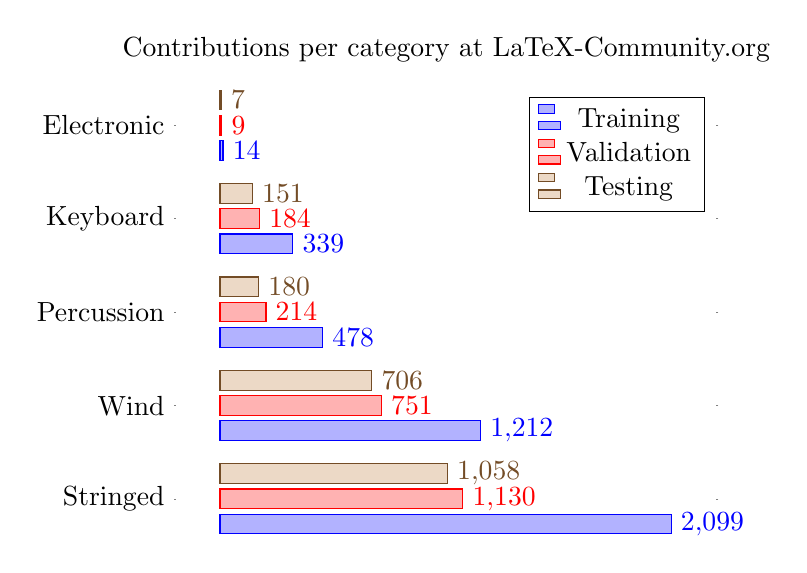
\begin{tikzpicture}
  \begin{axis}[title  = Contributions per category
                          at LaTeX-Community.org,
    xbar,
    bar width=.25cm,
    y axis line style = { opacity = 0 },
    axis x line       = none,
    tickwidth         = 0.8pt,
    symbolic y coords = {Stringed, Wind, Percussion,Keyboard, Electronic},
    nodes near coords,
  ]
\addplot coordinates {(2099,Stringed) (1212,Wind) (478,Percussion) (339,Keyboard) (14,Electronic)};
\addplot coordinates {(1130,Stringed) (751,Wind) (214,Percussion) (184,Keyboard) (9,Electronic)};
\addplot coordinates {(1058,Stringed) (706,Wind) (180,Percussion) (151,Keyboard) (7,Electronic)};
\legend{Training,Validation,Testing}

\end{axis}
\end{tikzpicture}

\iffalse
\end{axis}
\end{tikzpicture}
\fi

	\caption{A visual representation of the distribution of the hypernym classes that are present within \texttt{Minerva-0} and that define the \texttt{Minerva-Hypernym} benchmark.}
	\label{fig:hypernym_distribution}
\end{figure}


\section{Benchmarking}
\label{sec:benchmarking}

While MINERVA has been created with the primary intention of serving as a novel dataset for object detection, it can nevertheless still be used for testing the classification performance of convolutional neural networks as well. Although this task is certainly easier than the one of object detection, it is still of high interest as it provides a novel benchmark for further characterizing the transfer learning properties of neural networks that we started studying in the previous chapter. Therefore, we hereafter report results both for \textcolor{RoyalBlue}{classification} experiments as for \textcolor{RoyalBlue}{object detection} experiments. In the first section we consider the target task $\mathcal{T}_T$ of classifying the bounding boxes that have been annotated in MINERVA as standalone images, while in the second section we aim at both detecting and classifying the content of the potentially detected bounding boxes. We hereafter describe the experimental protocol used for both sets of experiments into detail.

\subsection{Classification}
The experimental setup used for the classification experiments largely builds on top of the study that we presented in Chapter \ref{ch:tl_natural_to_non_natural}. We continue to explore whether popular neural architectures, that have obtained state of the art results on the ImageNet benchmark, are able to perform equally well when they are trained on datasets of non natural images. To this end, we again consider the well known VGG19 \cite{simonyan2014very}, InceptionV3 \cite{szegedy2016rethinking} and ResNet50 \cite{xie2017aggregated} neural architectures. As done in the previous chapter we keep investigating the effect that different weight initialization strategies have on the final performance of the networks, with the goal of further characterizing the potential benefits that can come from adopting transfer learning. Specifically, we train the three considered neural architectures by following three different initalization strategies: `random" which simply initializes the model's parameters after following a initalization strategy, `ImageNet" which instead uses the weights that have been obtained after training the networks on the ImageNet source task $\mathcal{T}_S$, and `RijksNet" which are the models we trained both on the ImageNet dataset and on the Rijksmuseum collection, and that were also used for the final experiments of the previous chapter. For this study we only fine tune the networks, while we do not explore their performance when they are used as off the shelf feature extractors. We train all networks with the Adam optimizer \cite{kingma2014adam} and by using an initial learning rate of $0.001$. As already done for the previous study, we again controlled the training process by using early stopping and by interrupting the training regime as soon as the validation loss did not decrease for five epochs in a row. Naturally, all networks minimize the categorical crossentropy loss function.

\subsection{Object Detection}
\label{sec:object_detection_exp}

For this set of experiments we explore the performance of a YOLO object detector \cite{redmon2017yolo9000}, a popular neural architecture that has obtained state of the art results on the MS-COCO object detection benchmark. YOLO treats the task of object detection as a standard regression problem by dividing an image into a $S\times S$ grid and by predicting for each grid cell $B$ bounding boxes and $C$ class probabilities. The main assumption behind YOLO is that any of the $S\times S$ cells contains at most the center of one single object, therefore for every image, cell index $i=1,...,S\times S$, predicted box $j=1,...,B$ and class index $c=1,...,C$ we have the following components: 

\begin{itemize}
	\item $\mathbb{1}_{i}^\text{obj}$ which is $1$ if there is an object in cell $i$, and $0$ otherwise;
	\item $\mathbb{1}_{i,j}^\text{obj}$ which is $1$ if there is an object in cell $i$ and predicted box $j$ that is the most fitting one, whereas is $0$ otherwise; 
	\item $p_{i,c}$ which is $1$ if there in an object of class $c$ in cell $i$, and 0 otherwise;
	\item $x_i,y_i,w_i,h_i$ which are the coordinates of an annotated bounding box that are defined only if $\mathbb{1}_{i}^{\text{obj}}=1$;
	\item $c_{i,j}$ which is the IoU between the predicted box and the ground truth target.
\end{itemize}

At training, YOLO computes the value of the $\mathbb{1}_{i,j}^{\text{obj}}$ for each image together with the respective $c_{i,j}$, and then minimizes the following multi-part loss function:

\begin{aligned}
& \lambda_\text{coord} \sum_{i=1}^{S \times S} \sum_{j=1}^B \mathbb{1}_{i,j}^\text{obj} \left( (x_i - \hat{x}_{i,j})^2 + (y_i - \hat{y}_{i,j})^2 + (\sqrt{w_i} - \sqrt{\hat{w}_{i,j}})^2 + (\sqrt{h_i} - \sqrt{\hat{h}_{i,j}})^2\right)\\\\
& + \lambda_\text{obj} \sum_{i=1}^{S \times S} \sum_{j=1}^B \mathbb{1}_{i,j}^\text{obj} (c_{i,j} - \hat{c}_{i,j})^2 + \lambda_\text{noobj} \sum_{i=1}^{S \times S} \sum_{j=1}^B (1-\mathbb{1}_{i,j}^\text{obj}) \hat{c}_{i,j}^2  \\\\
& + \lambda_\text{classes} \sum_{i=1}^{S \times S} \mathbb{1}_i^\text{obj} \sum_{c=1}^C (p_{i,c} - \hat{p}_{i,c})^2 
\end{aligned}

where $\hat{p}{i,c}$, $\hat{x}{i,j}$, $\hat{y}{i,j}$, $\hat{w}{i,j}$, $\hat{h}{i,j}$ and $\hat{c}{i,j}$ are the predictions of the network.

In our experiments we use the YOLO-V3 version of the network introduced by \citet{redmon2018yolov3} and initialize it with the weights that are obtained after training the network on the MS-COCO dataset. Regarding the stochastic optimization procedure we use two different optimizers: we train the network with the Adam optimizer for the first 10 epochs, while we then use the RMSprop optimizer for the remaining training epochs, which are again controlled through early stopping. To assess the final performance of the model, we follow an evaluation protocol that is typical for object detection problems in CV \cite{lin2014microsoft}. Each detected bounding box is compared to the bounding box which has been annotated on the \texttt{Cytomine} platform. We only consider bounding boxes for which the confidence level is $\geq 0.05$, following the protocol established by \citet{everingham2010pascal}. We then compute the "Intersection over Union" (IoU) for measuring how much the detected bounding-boxes differ from the ground-truth ones. To assess whether a prediction can be considered as a true positive or a false positive, we define two, increasingly restrictive metrics: first, IoU $\geq10$ and, secondly, IoU $\geq50$. This approach is inspired by the work of \citet{gonthier2018weakly}, where the authors report results for both IoU thresholds when assessing the performance of their weakly supervised learning system on the IconArt dataset.

\section{Results}
\label{sec:minerva_results}

\subsection{Quantitative Analysis}
\label{sec:quantitative_analysis}
\paragraph{Classification}

We start by discussing the results obtained with our classification experiments. The performance of all models is reported in Tables \ref{table:minerva_no_tl_results}, \ref{table:minerva_tl_results} and \ref{table:minerva_rijks_results}, where we present the accuracy that the networks have obtained on the different Minerva testing sets, together with their respective F-1 scores. To this end for a given class $c$, a ground truth label $y$ and a model's prediction $\hat{y}$, let us introduce the notions of precision and recall. The first is computed as:
\begin{equation}
	\text{P}(c)=p(y=c|\hat{y}=c)=\frac{TP}{TP+FP},
\end{equation}
while the latter as
\begin{equation}
	\text{R}(c)=p(y=c|\hat{y}=c)=\frac{TP}{TP+FN}.
\end{equation}
Both quantities can be used for computing the F-1 score as follows:
\begin{equation}
	\text{F-1}(c)=2 \cdot \frac{\text{P}(c)\cdot\text{R}(c)}{\text{P}+\text{R}}.
\end{equation}
Similarly to the results reported in Chapter \ref{ch:tl_natural_to_non_natural} we again report the best performing architecture in a green cell, while the second best performing model in a yellow one.  

We can start by observing that among all the results presented in the three different tables, the best performing models are either the ones reported in Table \ref{table:minerva_tl_results}, or the ones presented in Table \ref{table:minerva_rijks_results}. This confirms the results that were presented in the previous chapter: fine tuning pre-trained models yields significantly better results that training models from scratch, even when the source and the target tasks can be particularly different (as is the case for musical instruments classification). While the results of this study confirm the conclusions that were drawn at the end of Chapter \ref{ch:tl_natural_to_non_natural}, they also provide some additional insights that were not observed before. First, it appears that the best performing architecture is not ResNet50 anymore, but rather the arguably older InceptionV3, a result which seems to suggest that there is no overall best performing architecture for all target tasks $\mathcal{T}_T$, and that the best architecture is highly problem dependent. Second, and perhaps arguably more surprising, we can also see that differently from what was observed in the last experiment in Chapter \ref{ch:tl_natural_to_non_natural}, it appears to be more beneficial to transfer models pre-trained on ImageNet only, instead of models that are additionally trained on the Rjksmuseum collection. Indeed, as can be observed by the results presented in Tables \ref{table:minerva_tl_results} and \ref{table:minerva_rijks_results}, the latter pre-training strategy outperforms the first one only when the ResNet50 and the InceptionV3 architectures are trained on the \texttt{Minerva-5} benchmark. These results can be explained as follows: in Chapter \ref{ch:tl_natural_to_non_natural} the target task $\mathcal{T}_T$ tackled with a model pre-trained on the Rijksmuseum collection corresponded to the original source task $\mathcal{T}_S$ (classification of `types" and `artists"). In these experiments however, albeit coming from similar domains, the considered source task $\mathcal{T}_S$ and target task $\mathcal{T}_T$ are unrelated, which could work in favor of an arguably more general ImageNet weight initialization.


\begin{table}[ht!]
	\caption{Results obtained when classifying the bounding boxes of the three different MINERVA benchmarks with models that do not come as pre-trained on any sort of source task $\mathcal{T}_S$. We can see that their performance is significantly worse than the one that is obtained when the same models come as pre-trained (see Table \ref{table:minerva_tl_results} and Table \ref{table:minerva_rijks_results}).}
\resizebox{\columnwidth}{!}{%
	\begin{tabular}{l|cc|cc|cc} \hline
	$\mathcal{T}_T$ &  \multicolumn{2}{c}{ResNet50} & \multicolumn{2}{|c|}{InceptionV3} & \multicolumn{2}{c}{VGG19}\\
			& Accuracy ($\%$) & F1 & Accuracy ($\%$) & F1 & Accuracy $(\%)$ & F1 \\\hline \hline
	\texttt{Minerva-Hypernym} & 50.33 & 13.39 & 51.80 & 14.02 & 50.12 & 13.12 \\
	\texttt{Minerva-5} & 40.83  & 21.88 & 40.49 & 21.65 & 41.26 & 22.01\\
	\texttt{Minerva-10} & 32.85 & 0.09  & 32.18 & 0.09 & 19.72 & 0.03 \\
\hline
\end{tabular}
%
}
\label{table:minerva_no_tl_results}
\end{table}



\begin{table}[ht!]
	\caption{Results obtained when classifying the bounding boxes of the three different MINERVA benchmarks after adapting transfer learning and considering the ImageNet dataset as the only source task $\mathcal{T}_S$. We observe that, compared to the results presented in Table \ref{table:minerva_no_tl_results}, this approach yields significant benefits, therefore confirming the results presented in Chapter \ref{ch:tl_natural_to_non_natural}.}
\resizebox{\columnwidth}{!}{%
	\begin{tabular}{l|cc|cc|cc} \hline
	$\mathcal{T}_T$ &  \multicolumn{2}{c}{ResNet50} & \multicolumn{2}{|c|}{InceptionV3} & \multicolumn{2}{c}{VGG19}\\
			& Accuracy ($\%$) & F1 & Accuracy ($\%$) & F1 & Accuracy $(\%)$ & F1 \\\hline \hline
	\texttt{Minerva-Hypernym} & \cellcolor{yellow!25}{76.64} & \cellcolor{yellow!25}{58.56} & \cellcolor{green!25}{79.40} & \cellcolor{green!25}{60.07} & 76.54 & 57.39 \\
	\texttt{Minerva-5} & 60.41  & 49.10 & 72.06 & 68.89 & 70.43 & 68.42\\
	\texttt{Minerva-10} & 55.37 & 41.65  & \cellcolor{green!25}{60.1} & \cellcolor{green!25}{45.12} & 44.22 & 40.12 \\
\hline
\end{tabular}
%
}
\label{table:minerva_tl_results}
\end{table}


\begin{table}[ht!]
	\caption{Results obtained when classifying the bounding boxes of the three different MINERVA benchmarks after adapting transfer learning and considering the ImageNet and the Rijksmuseum collection as source domains $\mathcal{D}_S$. Similarly to what was observed in Table \ref{table:minerva_tl_results}, we can again see that transfer learning yields significant benefits although this weight initialization strategy does mostly not outperform the more common ImageNet one.}
\resizebox{\columnwidth}{!}{%
	\begin{tabular}{l|cc|cc|cc} \hline
	$\mathcal{T}_T$ &  \multicolumn{2}{c}{ResNet50} & \multicolumn{2}{|c|}{InceptionV3} & \multicolumn{2}{c}{VGG19}\\
			& Accuracy ($\%$) & F1 & Accuracy ($\%$) & F1 & Accuracy $(\%)$ & F1 \\\hline \hline
	\texttt{Minerva-Hypernym} & 72.26 & 52.66 & \cellcolor{green!25}{75.80} & \cellcolor{green!25}{57.03} & 66.41 & 40.35 \\
	\texttt{Minerva-5} & 68.71  & 64.10 & \cellcolor{green!25}{73.66} & \cellcolor{green!25}{70.29} & 48.33 & 33.92\\
	\texttt{Minerva-10} & 52.85 & 41.55  & \cellcolor{green!25}{55.51} & \cellcolor{green!25}{44.77} & 37.52 & 15.22 \\
\hline
\end{tabular}
%
}
\label{table:minerva_rijks_results}
\end{table}


\paragraph{Object Detection}
The results for this set of experiments are reported in terms of average precision as for each class we report the area under the precision-recall curve that is obtained by setting IoU $\geq10$ and $\geq50$ as explained in Sec. \ref{sec:object_detection_exp}. We start by discussing the performance that is obtained after fine-tuning a pre-trained YOLO-V3 model on the \texttt{Minerva-0} benchmark, where as a reminder, the goal is that of simply detecting a musical instrument within an image without classifying it. For an IoU $\geq 10$ we report an average precision of $35.33\%$, while for an IoU $\geq 50$ a final score of $22.31\%$. Both scores demonstrate that the model is successfully able to detect the musical instruments within MINERVA and that, on this task, its performance is on par with the one that is reported on more common object detection benchmarks \cite{}. More specifically, the model detects an instrument $1386$ times, out of which when an IoU $\geq 10$ is considered, $878$ detections correspond to true positives, whereas $508$ detections are false positives. Naturally, the performance of the model decreases when an IoU $\geq 50$ is considered, as the amount of true positive detections decreases to $648$ and the number of false positives increases to $738$.

We report a similar quantitative analysis for the \texttt{Minerva-Hypernym}, \texttt{Minerva-5} and \texttt{Minerva-10} benchmarks. We do this in Tables \ref{table:minerva_detection_hypernym}, \ref{table:minerva_5_detection} and \ref{table:minerva_10_detection} where we present the different average precision scores, and in Figures \ref{fig:detection_experiment_2}, \ref{fig:detection_experiment_3} and \ref{fig:detection_experiment_4}, where we visualize the true vs false positives detections. We can see that out of these three benchmarks, the \texttt{Minerva-Hypernym} one appears to be the most challenging one as it results into the worst performing models independently from which IoU threshold is considered. We can observe from Fig. \ref{fig:detection_experiment_2} that the model is able to detect `stringed instruments" successfully, whereas its performance in detecting the remaining four hypernyms of the dataset is drastically worse. When it comes to the \texttt{Minerva-5} benchmark we can observe from Table \ref{table:minerva_5_detection} that the model is able to successfully detect three instruments out of the five instruments which constitute this benchmark, namely `Harps', `Lutes", and `Violins". These results are only second to the ones obtained on \texttt{Minerva-0}, although the considered target task $\mathcal{T}_T$ is now significantly harder. Similar detections have been obtained after fine-tuning the model on the \texttt{Minerva-10}benchmark, here we can again observe (see Table \ref{table:minerva_10_detections} and Fig. \ref{fig:detection_experiment_4}) that the network is able to only successfully detect the first three most occurring instruments of the dataset, whereas for the `Horn", `Bagpipe" `Rebec" and `Lyre" classes no detections are made. 

\begin{table}[ht!]
	\caption{Average Precision ($\%$) obtained when fine-tuning a pre-trained YOLO-V3 object detector on the \texttt{Minerva-Hypernyms} dataset. We can observe that satisfying results are obtained for both IoU thresholds when it comes to the detection of stringed instruments, whereas detecting the remaining four hypernyms of MINERVA appears to be much more challenging.}
\resizebox{\columnwidth}{!}{%	
	\begin{tabular}{c|c|c|c|c|c||c}\hline
		& Stringed & Wind & Percussion & Keyboard & Electronic & Mean\\ 
	AP IoU $\geq10$ & 28.22         & 4.58      & 2.55           & 7.36  & 0   &  6.03  \\
	AP IoU $\geq50$ & 20.95         &  2.91    &  1.84          &  4.47       & 0 & 8.54 
\end{tabular}
%
}
\label{table:minerva_detection_hypernyms}
\end{table}


\begin{table}[ht!]
	\caption{Average Precision ($\%$) obtained on the \texttt{ Minerva-5} benchmark. We can observe that the fine-tuned model successfully detects `Harps", `Lutes" and `Violins", whereas the detection of `Shawns" and `Trumpets" can be improved.}
\resizebox{\columnwidth}{!}{%	
	\begin{tabular}{c|c|c|c|c|c||c}\hline
		& Harp & Lute & Violin & Shawn & Trumpet & Mean\\ \hline \hline 
	AP IoU $\geq10$ & 55.60         & 36.51      & 12.21           & 1.75 & 1.3   &  21.47  \\
	AP IoU $\geq50$ & 46.80         &  26.93    &  7.64          &  1.01       & 1.07 & 16.69 
\end{tabular}
%
}
\label{table:minerva_5_detection}
\end{table}


\begin{table}
	\caption{Average Precision ($\%$) obtained on the \texttt{Minerva-10} benchmark. Similarly to what was presented in Table \ref{table:minerva_5_detection}, we can again observe that the model successfully detects the first three most occurring instruments within the dataset, whereas it appears to perform poorly on the remaining instrument classes.}
\resizebox{\columnwidth}{!}{%	
	\begin{tabular}{c|c|c|c|c|c|c|c|c|c|c||c}\hline
		& Harp & Lute & Violin & Shawn & Trumpet  & Organ & Rebec & Lyre & Horn & Bagpipe & Mean\\ 
	AP IoU $\geq10$ &  46.88         &  33.74    &  6.73          &  0.59       & 1.83 & 6.1 & 0 & 0 & 0 & 0 & 9.58  \\
	AP IoU $\geq50$ & 39.81         &  25.40    &  4.82          &  0.59       & 0.14 & 6.1 & 0 & 0 & 0 & 0 & 7.68 
\end{tabular}
%
}
\label{table:minerva_10_detection}
\end{table}


\begin{figure}[htb!]
	\scalebox{0.8}{\begin{minipage}{.5\textwidth}
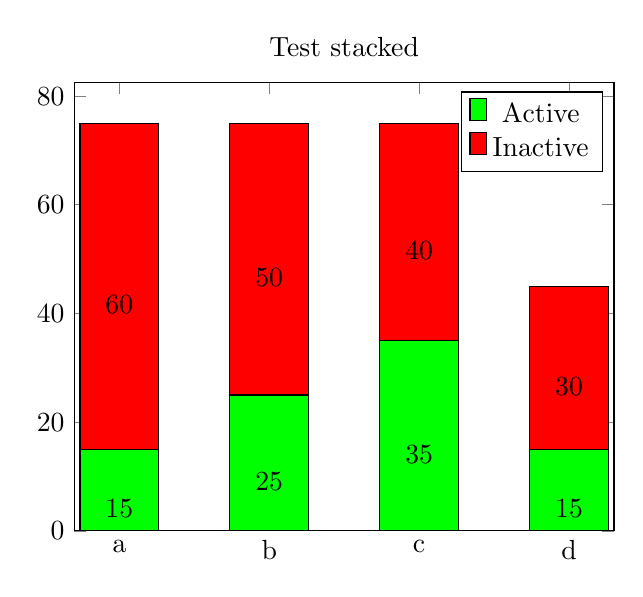
\begin{tikzpicture}
  \begin{axis}[
    title={Test stacked},
    ybar stacked, ymin=0,  
    bar width=10mm,
    symbolic x coords={a,b,c,d},
    xtick=data,
    nodes near coords, 
    nodes near coords align={anchor=north},%Move values in bar
    every node near coord/.style={
    },
  ]
  %Active
  \addplot [fill=green] coordinates {
({a},15)
({b},25)
({c},35)
({d},15)};
  %Inactive
  \addplot [fill=red] coordinates {
({a},60)
({b},50)
({c},40)
({d},30)};
  \legend{Active,Inactive}
  \end{axis}
 \end{tikzpicture}
 \end{minipage}
 \hspace{2.5cm}
\begin{minipage}{.5\textwidth}
 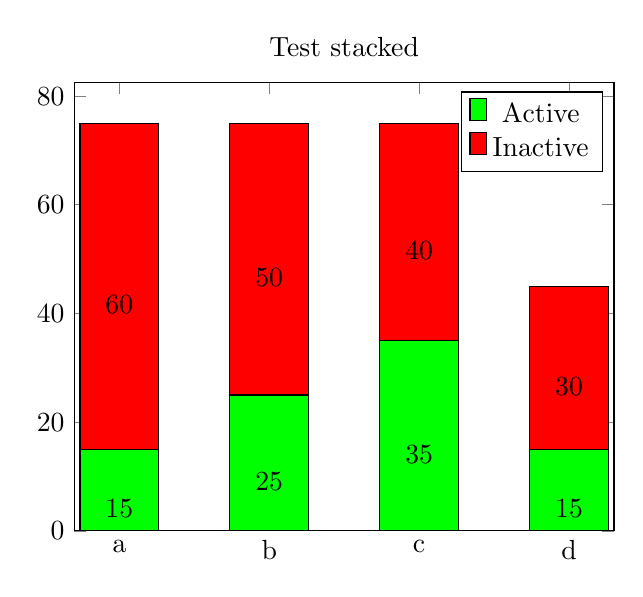
\begin{tikzpicture}
  \begin{axis}[
    title={Test stacked},
    ybar stacked, ymin=0,  
    bar width=10mm,
    symbolic x coords={a,b,c,d},
    xtick=data,
    nodes near coords, 
    nodes near coords align={anchor=north},%Move values in bar
    every node near coord/.style={
    },
  ]
  %Active
  \addplot [fill=green] coordinates {
({a},15)
({b},25)
({c},35)
({d},15)};
  %Inactive
  \addplot [fill=red] coordinates {
({a},60)
({b},50)
({c},40)
({d},30)};
  \legend{Active,Inactive}
  \end{axis}
 \end{tikzpicture}
 \end{minipage}

}
	\caption{True Positive (TP) vs False Positive (FP) analysis on the \texttt{Minerva-Hypernym} benchmark for IoU $\geq10$ and IoU $\geq50$.}
	\label{fig:detection_experiment_2}
\end{figure}



\begin{figure}[htb!]
	\scalebox{0.8}{\begin{minipage}{.5\textwidth}
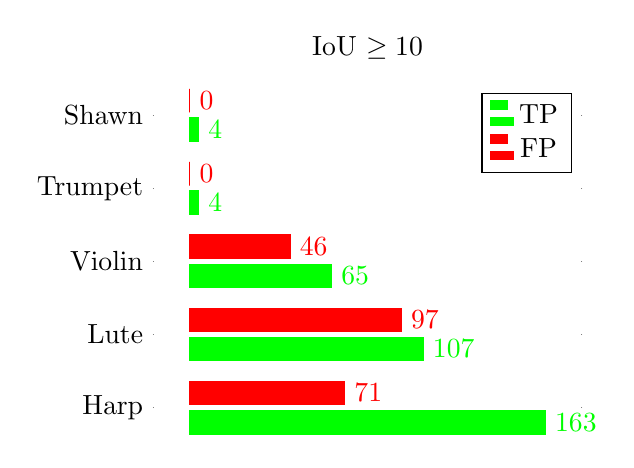
\begin{tikzpicture}
  \begin{axis}[title  = IoU $\geq 10$,
    xbar,
    bar width=.3cm,
    y axis line style = { opacity = 0 },
    axis x line       = none,
    tickwidth         = 0.5pt,
    width=7cm,
    symbolic y coords = {Harp, Lute, Violin, Trumpet, Shawn},
    ytick= data,
    nodes near coords,
  ]
  \addplot [color=green,fill ] coordinates {(163,Harp) (107,Lute) (65,Violin) (4,Trumpet) (4,Shawn)};
  \addplot [color=red,fill] coordinates {(71,Harp) (97,Lute) (46,Violin) (0,Trumpet) (0,Shawn)};
\legend{TP,FP}
\end{axis}
\end{tikzpicture}
 \end{minipage}
 \hspace{3cm}
\begin{minipage}{.5\textwidth}
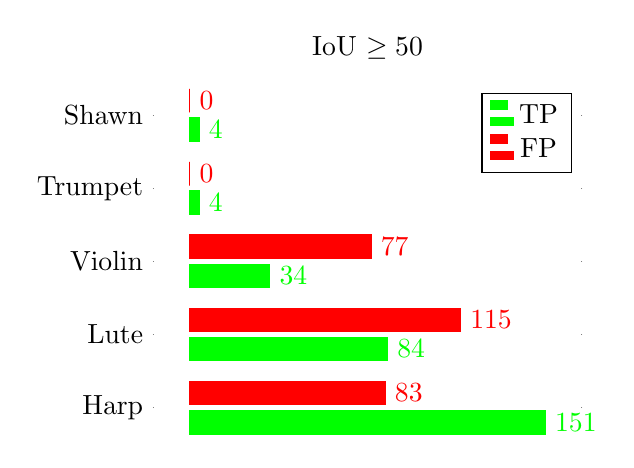
\begin{tikzpicture}
  \begin{axis}[title  = IoU $\geq 50$,
    xbar,
    bar width=.3cm,
    y axis line style = { opacity = 0 },
    axis x line       = none,
    tickwidth         = 0.5pt,
    width=7cm,
    symbolic y coords = {Harp, Lute, Violin, Trumpet, Shawn},
    ytick=data,
    nodes near coords,
  ]
  \addplot [color=green,fill] coordinates {(151,Harp) (84,Lute) (34,Violin) (4,Trumpet) (4,Shawn)};
  \addplot [color=red,fill] coordinates {(83,Harp) (115,Lute) (77,Violin) (0,Trumpet) (0,Shawn)};
\legend{TP,FP}

\end{axis}
\end{tikzpicture}
 \end{minipage}
 

}
	\caption{True Positive (TP) vs False Positive (FP) analysis on the \texttt{Minerva-5} benchmark for IoU $\geq10$ and IoU $\geq50$.}
	\label{fig:detection_experiment_3}
\end{figure}


\begin{figure}[htb!]
	\scalebox{0.8}{\begin{minipage}{.5\textwidth}
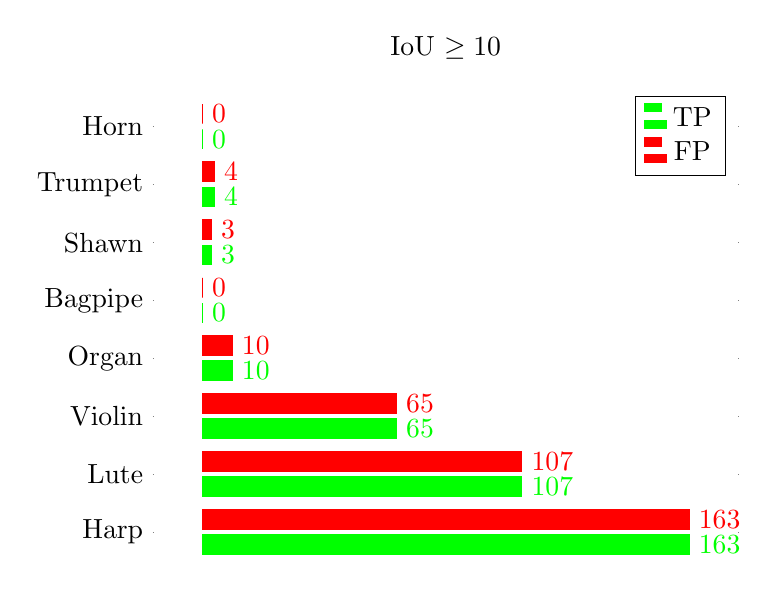
\begin{tikzpicture}
  \begin{axis}[title  = IoU $\geq 10$,
    xbar,
    bar width=.25cm,
    y axis line style = { opacity = 0 },
    axis x line       = none,
    tickwidth         = 0.3pt,
    width=9cm,
    symbolic y coords = {Harp, Lute, Violin, Organ, Bagpipe, Shawn, Trumpet, Horn},
    ytick= data,
    nodes near coords,
  ]
  \addplot [color=green,fill ] coordinates {(163,Harp) (107,Lute) (65,Violin) (10,Organ) (0,Bagpipe) (3,Shawn) (4,Trumpet) (0,Horn)};
  \addplot [color=red,fill] coordinates {(163,Harp) (107,Lute) (65,Violin) (10,Organ) (0,Bagpipe) (3,Shawn) (4,Trumpet) (0,Horn)};
\legend{TP,FP}
\end{axis}
\end{tikzpicture}
 \end{minipage}
 \hspace{3cm}
\begin{minipage}{.5\textwidth}
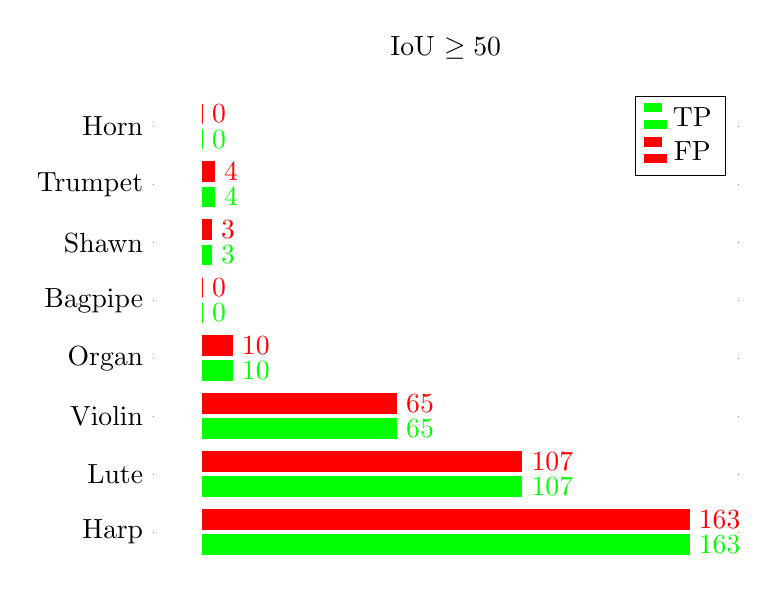
\begin{tikzpicture}
  \begin{axis}[title  = IoU $\geq 50$,
    xbar,
    bar width=.25cm,
    y axis line style = { opacity = 0 },
    axis x line       = none,
    tickwidth         = 0.3pt,
    width=9cm,
    symbolic y coords = {Harp, Lute, Violin, Organ, Bagpipe, Shawn, Trumpet, Horn},
    ytick=data,
    nodes near coords,
  ]
  \addplot [color=green,fill] coordinates {(163,Harp) (107,Lute) (65,Violin) (10,Organ) (0,Bagpipe) (3,Shawn) (4,Trumpet) (0,Horn)};
  \addplot [color=red,fill] coordinates {(163,Harp) (107,Lute) (65,Violin) (10,Organ) (0,Bagpipe) (3,Shawn) (4,Trumpet) (0,Horn)};
\legend{TP,FP}

\end{axis}
\end{tikzpicture}
 \end{minipage}
 

}
	\caption{True Positive (TP) vs False Positive (FP) analysis on the \texttt{Minerva-Hypernym} benchmark for IoU $\geq10$ and IoU $\geq50$.}
	\label{fig:detection_experiment_4}
\end{figure}



\subsection{Qualitative Analysis}
\label{sec:qualitative_analysis}
We now characterize the performance of the aforementioned fine-tuned models from a qualitative perspective. 

\paragraph{Object Classification}
For the classification experiments we keep building on top of the study presented in the previous chapter, and perform a qualitative evaluation of the models that is based on the visualization of saliency maps, as this allows us to investigate which visual properties in the image are exploited by the networks for correctly classifying the instruments in MINERVA. We hereafter report saliency maps that are obtained after fine-tuning an ImageNet pre-trained ResNet50 model on the \texttt{Minerva-Hypernym} benchmark and that are computed with two, different, gradient-based techniques: Grad-CAM \cite{selvaraju2017grad} and Grad-CAM ++ \cite{chattopadhay2018grad}. Examples of computed saliencies are reported in Fig. \ref{fig:grad_cams}. We can observe that the model focuses on two broad types of regions within the image: properties of the instruments itself (which can be expected), but also the immediate context of the instruments, and more specifically the way they are operated, handled or presented. Let us for example consider the `stringed instruments" category: as can be seen from the images in the first and third row of Fig. \ref{fig:grad_cams}, the network happens to focus more on the strings of the instruments rather than on the, arguably more representative, resonance body of the instrument (which is however of interest in the second row of images). When it comes to the `percussion instrument" represented in the forth row, and the `wind instrument" represented in the last row, we can again observe that the model considers the fingers handling the instruments at least as important as the instruments themselves.  

While saliency maps are indeed able to produce appealing visual explanations of the performance of neural networks, it is also worth noting that the output of these methods should also be critically assessed. As reported by \citet{alqaraawi2020evaluating} saliency maps do not always necessarily explain the model's predictions, and there is a large body of work questioning their reliability \cite{simonyan2013deep,arun2020assessing,saporta2021deep}. Nevertheless they can still be interesting to visually inspect, as long as the resulting saliencies are taken with a grain of sand. 

\begin{figure}[ht!]
\centering
  \includegraphics[width=\linewidth]{./Images/Chapter05/grad_cams}
  \caption{Saliency maps obtained after fine-tuning an ImageNet pre-trained ResNet50 on the \texttt{Minerva-Hypernym} benchmark. The first image corresponds to the original image, while the second and fourth images, and the third and fifth images, respectively report the performance of the Grad-CAM and Grad-CAM ++ methods.}
  \label{fig:grad_cams}
\end{figure}


\paragraph{Object Detection}
Regarding the models trained for object detection, we visually investigate the quality of the predictions on the IconArt dataset \cite{gonthier2018weakly}, a database of $\approx 6000$ paintings that has been collected with the aim of detecting classes that are specific to the analysis of artworks. Among such classes IconArt tackles the detection of `angels", `Jesus" and `Mary", or more simply `ruins". IconArt, however, does not come with any ground truth labels that are suitable for the task of instruments detection, as the dataset has been built for different purposes. Yet, musical instruments might still be depicted within its images, and trying to detect them corresponds to a nice proof of concept that can show the benefits of deploying Minerva pre-trained models to different artistic collections. In Fig. \ref{fig:wikiart_detections} we show some successful examples of detections that were obtained after testing the performance of a YOLO-V3 model that was fine-tuned on the \texttt{Minerva-Hypernym} benchmark. We see that the model is indeed able to successfully detect musical instruments within this new artistic collection, a result that can be exploited by art historians that are interested in the study of musical instruments .   

\begin{figure}[ht!]
\centering
  \includegraphics[width=\linewidth]{./Images/Chapter05/wikiart_detections}
  \caption{Some examples of successful detections that have been obtained on the IconArt dataset with a model fine-tuned on the \texttt{Minerva-Hypernym} benchmark.}
  \label{fig:wikiart_detections}
\end{figure}

While these results are certainly nice and encouraging, it is arguably of even larger interest analyzing the model's detections which are erroneous. To this end, we have manually identified the incorrect model's predictions, and grouped them into different categories. This process resulted into novel insights that, at least in part, explain the performance of the models that we have quantitatively assessed in Sec. \ref{sec:quantitative_analysis}.
First and foremost, we have noticed that the model strongly gravitates towards the detection of `stringed instruments" (a result which was already observed in Fig. \ref{fig:detection_experiment_2}). We believe that such detections are driven by two main reasons: the large presence of dual, conic contour curves of naked women's bodies, which are reminiscent of the resonance box of guitar-like instruments (see Fig. \ref{fig:false_positives_1}), and the presence of book-like objects that, just as instruments, are mostly depicted next to hands and fingers (see Fig. \ref{fig:false_positives_4}). We have then also observed that long, often martial objects such as swords, arrows and spears are mistakenly detected as `wind instruments". We believe that the reason for this is that the shape between such objects and the one of instruments like `shawns", is very similar, and sometimes even hard to distinguish for the human eye (see Fig. \ref{fig:false_positives_2}).
Lastly we have noticed that musical instruments are often mistakenly detected when regular patterns or parallel grids of straight lines (e.g folds in clothing or wheel spokes) are present within the images. We hypothesize that the model associates these patterns to the presence of strings (see Fig. \ref{fig:false_positives_3}) within stringed instruments. 

\begin{figure}[ht!]
\centering
  \includegraphics[width=\linewidth]{./Images/Chapter05/false_positives_1}
  \caption{Examples of false detections of `stringed instruments" within some images representing `nudity" that are part of the IconArt dataset.}
  \label{fig:false_positives_1}
\end{figure}

\begin{figure}[ht!]
\centering
  \includegraphics[width=\linewidth]{./Images/Chapter05/false_positives_4}
  \caption{Additional examples of false detections of `stringed instruments" that are triggered by the presence of objects close to hands and fingers.}
  \label{fig:false_positives_4}
\end{figure}

\begin{figure}[ht!]
\centering
  \includegraphics[width=\linewidth]{./Images/Chapter05/false_positives_2}
  \caption{Examples of false detections that are due to the strong resemblance between long martial objects and (mostly) `wind instruments".}
  \label{fig:false_positives_2}
\end{figure}


\begin{figure}[ht!]
\centering
  \includegraphics[width=\linewidth]{./Images/Chapter05/false_positives_3}
  \caption{Examples of geometrical patterns that mistakenly yield the detection of instruments.}
  \label{fig:false_positives_3}
\end{figure}



\section{Discussion and Critical Analysis}
\label{sec:discussion}
In this chapter we have introduced MINERVA, the first sizable benchmark dataset for the identification and detection of musical instruments in unrestricted, digitized images from the realm of the visual arts. We hope that this dataset can serve as a novel test-bed for the computer vision community as it provides, at least in part, a solution to some of the challenges that currently define the field (see Sec. \ref{sec:introduction}). Our benchmark experiments have highlighted the feasibility of our newly proposed classification and object detection tasks, and served us for further characterizing the degree of transferability of pre-trained convolutional neural networks. While, when it comes to the classification experiments presented in the first part of Sec. \ref{sec:quantitative_analysis}, the obtained results are lower in terms of accuracy when compared to the classification tasks that we tackled in the previous chapter, they nevertheless provide strong evidence in favor of adapting transfer learning. At the same time these experiments also show how challenging the simple task of image classification can be, as we believe there is definitively room for improving the results presented in Tables \ref{table:minerva_tl_results} and \ref{table:minerva_rijks_results}. Similarly, the results presented in the second part of Sec. \ref{sec:quantitative_analysis} show that it is equally possible to transfer models that have originally been built for the detection of objects in natural images, and to use them on non natural image distributions. We again believe that albeit satisfying results on MINERVA have been obtained by starting with a MS-COCO weight initialization, better performance than the one reported in Tables \ref{table:minerva_detection_hypernyms} \ref{table:minerva_5_detection} and \ref{table:minerva_10_detection} can be obtained. To this end, we recommend taking into account the qualitative analysis that we presented in Sec. \ref{sec:qualitative_analysis}. Overall our study is a first step towards the creation of novel, arguably more challenging computer vision test-beds, that we hope can be used for further characterizing the potential, and limitations, of modern state of the art neural networks. To this end, the methodological protocol that was used for the creation of MINERVA has already inspired the development of new datasets and experimental studies that will be briefly reviewed in the next section.

\section{Future Work: towards more benchmarks}
\label{sec:future_work}
